% Source of who_buys_because_of_the_coupon_proposal_zh_extended.pdf. Build in this folder with two runs of
%   xelatex -jobname=who_buys_because_of_the_coupon_proposal_zh_extended main.tex
% (fonts: TeX Gyre Termes/Heros, STIX Two Math, Noto Serif CJK SC) and copy who_buys_because_of_the_coupon_proposal_zh_extended.pdf to ../
\documentclass[a4paper,11pt]{article}
\usepackage{fontspec}
\setmainfont{TeX Gyre Termes}
\setsansfont{TeX Gyre Heros}
\newfontfamily\cjkfont{Noto Serif CJK SC}
\usepackage{amsmath}
\usepackage{unicode-math}
\setmathfont{STIXTwoMath-Regular.otf}
\usepackage[a4paper,top=2.5cm,bottom=2.4cm,left=2.6cm,right=2.6cm]{geometry}
\usepackage{graphicx,booktabs,array,threeparttable,pdfpages,fancyhdr,xurl}
\usepackage[font=small,labelsep=period,skip=4pt]{caption}
\usepackage[hidelinks,bookmarksnumbered=true,bookmarksopen=true]{hyperref}
\usepackage{titlesec}
\renewcommand{\floatpagefraction}{0.8}\renewcommand{\topfraction}{0.88}\renewcommand{\bottomfraction}{0.7}\renewcommand{\textfraction}{0.1}
\usepackage{etoolbox}\AtBeginEnvironment{thebibliography}{\small\linespread{1.05}\selectfont\setlength{\itemsep}{1pt}\setlength{\parskip}{0pt}}
\setlength{\emergencystretch}{3em}
\linespread{1.15}
\setlength{\parskip}{0.25em}
\titleformat{\section}{\large\bfseries}{E\arabic{section}}{0.8em}{}
\titleformat{\subsection}{\normalsize\bfseries}{E\arabic{section}.\arabic{subsection}}{0.6em}{}
\renewcommand{\thesection}{E\arabic{section}}
\renewcommand{\thefigure}{E\arabic{figure}}
\renewcommand{\thetable}{E\arabic{table}}
\renewcommand{\theequation}{E\arabic{equation}}
\setlength{\headheight}{15pt}\pagestyle{fancy}\fancyhf{}\renewcommand{\headrulewidth}{0.4pt}
\newcommand{\hd}[1]{\begin{tabular}[b]{@{}c@{}}#1\end{tabular}}
\newcommand{\exthead}[1]{\fancyhead[L]{\small #1}\fancyhead[R]{\small Part II\quad Post-competition extensions}\fancyfoot[C]{\small E-\thepage}}

\graphicspath{{../../figures/extension/}}
\hypersetup{pdftitle={Who buys because of the coupon -- extended edition}}
\begin{document}
\thispagestyle{empty}
\begin{center}
{\Large\bfseries Who Buys Because of the Coupon? Causal Uplift\\[0.2em] for Local-Services Coupon Budget Allocation}\\[0.7em]
{\large Extended edition --- note}
\end{center}
\vspace{0.8em}

This file has two parts. Part I is the proposal submitted to the 6th Meituan Business Analytics Elite Contest (15 pages, in Chinese), reproduced exactly as submitted. Part II, starting on page E-1, contains post-competition extensions written in November 2026.

The proposal's quantitative evaluation rests on a digital twin of 100\,000 users calibrated to quantiles of 197 real users and to effect sizes from the literature. The twin builds a persuadable segment into its data-generating process, so it cannot test the central claim of the proposal, namely that targeting by causal uplift beats targeting by purchase propensity. Part II tests that claim on public randomised marketing experiments instead. E1 reproduces the proposal's IPTW-weighted T-learner with isotonic calibration on the Hillstrom e-mail experiment and finds that uplift targeting does no better than response targeting. E2 compares seven targeting rules on three public randomised experiments with about 950\,000 customers in total. Whether uplift targeting pays depends on the marketing setting rather than on the learner, while the proposal's isotonic calibration step reduces the calibration error of the effect estimates in every split of all three experiments.

Every number in Part II can be reproduced with the scripts in the \texttt{extension/} folder of the code repository; result files are in \texttt{results/extension/}. The public data are downloaded at run time and are not redistributed.

\clearpage
\pdfbookmark[0]{Part I\quad Competition proposal (as submitted)}{part1}

\includepdf[pages=-]{../who_buys_because_of_the_coupon_proposal_zh.pdf}
\pdfbookmark[0]{Part II\quad Post-competition extensions}{part2}
\setcounter{page}{1}
\exthead{Who buys because of the coupon?}
\begin{center}{\Large\bfseries Part II\quad Post-competition extensions}\end{center}

The proposal argues that the coupon budget should move from predicting who will buy to estimating who buys because of the coupon, and it reports a 26.0\,\% lift in incremental orders on a digital twin. The twin writes into its data-generating process a persuadable segment with a baseline conversion rate of about 3\,\% that exceeds 30\,\% with a coupon. That structure is precisely the condition under which uplift targeting wins, so the lift cannot count as an independent test of the proposal's claim. The two extensions below use only public experiments with randomised treatment and no simulated data.

\section{A test on a real randomised experiment: does uplift targeting beat response targeting?}

\subsection{Data and design}
The Hillstrom e-mail experiment (MineThatData, 2008) randomly assigned 64\,000 customers with a purchase history to a men's e-mail, a women's e-mail or no e-mail, and recorded website visits and conversions over the following two weeks\cite{hillstrom2008}. The two e-mail groups are merged into one treatment group; visits are the primary outcome and conversions a secondary one. Each policy is trained on a random half of the sample and evaluated with the Qini curve on the other half, and the split is repeated 20 times. The policies are random targeting, a response model that predicts the probability of purchase, the T-learner uplift model of the proposal, and the full proposal, which adds IPTW-based isotonic calibration to the T-learner.

\subsection{Results}
Table~\ref{tab:mt-e1} reports the share of all incremental visits captured when the top 30\,\% of customers by predicted value are targeted. Both learned policies capture about 7 percentage points more than random targeting, but the uplift ranking and the response ranking perform almost identically: in paired comparisons the uplift ranking is better in only 10 of the 20 splits, with a mean difference of $+0.02$ percentage points, and conversions give the same conclusion.

\begin{table}[htbp]\centering\small
\caption{Targeting performance of each policy on the Hillstrom experiment (20 random splits).}\label{tab:mt-e1}
\begin{tabular}{lcc}\toprule
Policy (outcome: visit) & Share of incremental visits in top 30\,\% & Qini area\\\midrule
Random targeting & 28.8\,\% $\pm$ 3.2 & $-0.0002$\\
Response model (who will buy) & 36.1\,\% $\pm$ 2.5 & 0.0026\\
T-learner uplift model (who buys because of it) & 36.1\,\% $\pm$ 3.1 & 0.0025\\
Uplift model + IPTW isotonic calibration (proposal) & 36.1\,\% $\pm$ 3.1 & 0.0025\\\bottomrule
\end{tabular}
\end{table}

\begin{figure}[htbp]\centering
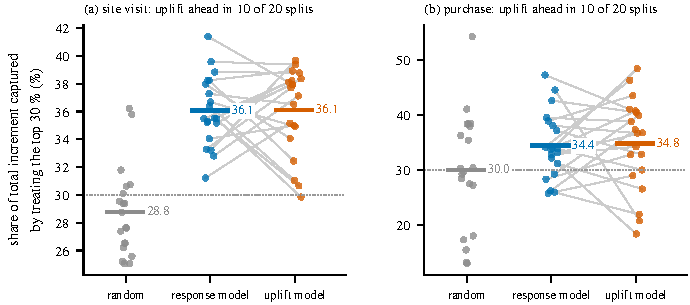
\includegraphics[width=0.62\textwidth]{figE1_hillstrom_targeting.pdf}
\caption{Cumulative incremental visits when customers of the Hillstrom experiment are targeted in the order of each ranking (Qini curves, 20 splits).}\label{fig:mt-e1}
\end{figure}

\subsection{Interpretation}
The result is not due to an absence of persuadable customers. The Spearman rank correlation between the estimated baseline visit rate and the estimated uplift is $-0.21$, and the two top-30\,\% lists overlap by only 46\,\%, so the two rankings do select different people. The limitation is estimation precision. Each training half contains about 21\,000 treated and 10\,700 control customers, and the T-learner estimates uplift as the difference of two independently fitted models, whose variance is large enough to cancel the difference between the rankings. Isotonic calibration is a monotone transformation: it changes the scale of the uplift estimates but not their order, so its value lies in budget allocation measured in money rather than in targeting itself. The 26\,\% lift reported by the proposal therefore depends on the heterogeneity built into the digital twin. Deployment would require a randomised hold-out group of sufficient size, an uplift learner with lower variance, and a pre-registered Qini comparison with the existing response model.

\section{Learner or setting? Seven targeting rules on three randomised experiments}

\subsection{Question and design}
E1 leaves two explanations open: either the T-learner is too noisy and an uplift learner with lower variance would beat response targeting, or the Hillstrom setting itself does not reward uplift targeting. To separate the two, E2 compares seven targeting rules on three public randomised experiments that cover the setting of the proposal, marketing contact followed by a purchase or a store visit (Table~\ref{tab:mt-data}). The 23 features of X5 are aggregated from 45.8 million receipt records before the campaign; Lenta uses the 191 customer features supplied with the dataset.

\begin{table}[htbp]\centering\small
\caption{The three public randomised experiments.}\label{tab:mt-data}\setlength{\tabcolsep}{4pt}
\begin{tabular}{lrrlr}\toprule
Experiment & Customers & \hd{Treated\\share} & Outcome & \hd{Average effect\\(control base rate)}\\\midrule
Hillstrom e-mail (2008) & 64\,000 & 2/3 & site visit in two weeks & $+6.1$ pp (10.6\,\%)\\
X5 RetailHero SMS (2019) & 200\,039 & 1/2 & purchase after campaign & $+3.3$ pp (60.3\,\%)\\
Lenta SMS (2020) & 687\,029 & 3/4 & store visit & $+0.75$ pp (10.3\,\%)\\\bottomrule
\end{tabular}
\end{table}

The seven rules are the response model, the S-learner, the T-learner, transformed-outcome regression\cite{athey2016}, the X-learner\cite{kunzel2019}, the DR-learner\cite{kennedy2023} and the causal forest\cite{athey2019}, all with the same gradient-boosting base learner. The T-learner is the ranking of the proposal, whose isotonic calibration does not change the order. Each rule is fitted on one half of a stratified 50/50 split and evaluated on the other, with 20, 10 and 5 repetitions for the three experiments. The metric is the Qini coefficient (the normalised Qini area of scikit-uplift; E1 reports the unnormalised area). Because the training sets of repeated random splits overlap, the 95\,\% confidence intervals of paired differences use the corrected resampled $t$-test of Nadeau and Bengio\cite{nadeau2003}, which inflates the between-split variance by the factor $(1/J+n_{\mathrm{test}}/n_{\mathrm{train}})$, where $J$ is the number of splits.

\subsection{Results}

\begin{table}[htbp]\centering\small
\caption{Qini coefficient of each targeting rule (mean over splits; bold marks the largest value in each experiment apart from random targeting).}\label{tab:mt-qini}
\begin{tabular}{lrrr}\toprule
Targeting rule & Hillstrom & X5 & Lenta\\\midrule
Response model (who will buy) & \textbf{0.0200} & $-0.0072$ & \textbf{0.0051}\\
S-learner & 0.0188 & 0.0153 & 0.0013\\
T-learner (the proposal's ranking) & 0.0141 & 0.0128 & 0.0036\\
Transformed-outcome regression & 0.0147 & 0.0138 & 0.0047\\
X-learner & 0.0192 & \textbf{0.0162} & 0.0039\\
DR-learner & 0.0169 & 0.0137 & 0.0017\\
Causal forest & 0.0174 & 0.0138 & 0.0004\\
Random & 0.0011 & 0.0013 & $-0.0014$\\\midrule
Share of uplift in top 30\,\% (response / best uplift learner) & 35\,\% / 35\,\% & 15\,\% / 61\,\% & 41\,\% / 45\,\%\\
T-learner calibration error, raw $\to$ isotonic (pp) & 3.0 $\to$ 1.0 & 2.7 $\to$ 0.9 & 1.6 $\to$ 0.4\\\bottomrule
\end{tabular}
\end{table}

\begin{figure}[htbp]\centering
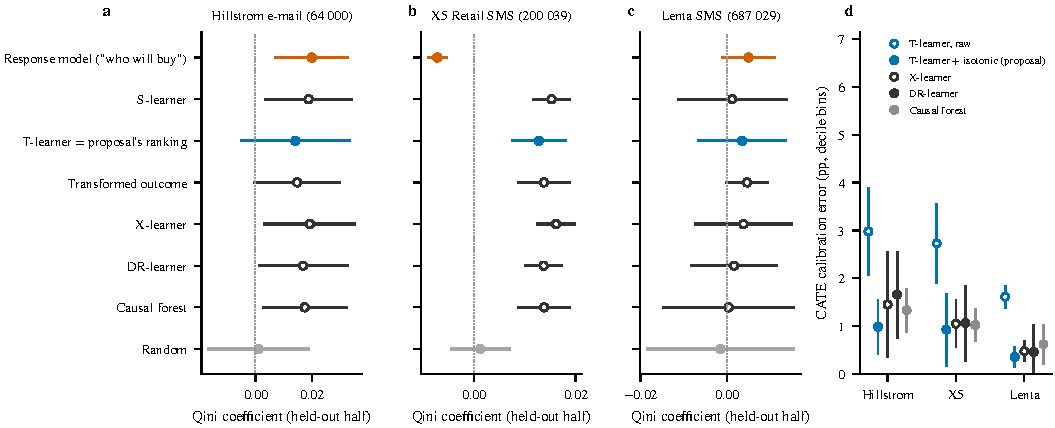
\includegraphics[width=\textwidth]{figE2_uplift_benchmark.pdf}
\caption{(a--c) Qini coefficient of each targeting rule on the held-out halves: points are means, bars the corrected 95\,\% intervals. (d) Calibration error of the uplift estimates computed over decile bins; filled blue points are the proposal's isotonic calibration.}\label{fig:mt-e2}
\end{figure}

Whether uplift targeting pays depends on the marketing setting, not on the choice of learner. In X5 the customers most likely to buy are exactly those least affected by the SMS: response targeting has a negative Qini coefficient, worse than random targeting, and its top 30\,\% contains only 15\,\% of all incremental purchases. All six uplift learners beat response targeting in all 10 splits, the X-learner by $+0.023$ (95\,\% confidence interval $[0.019, 0.028]$). In Hillstrom and Lenta the situation is reversed, and the response model is at least as good as the best uplift learner: the difference of the X-learner from the response model is $-0.0007$ ($[-0.0211, +0.0196]$) in Hillstrom, and that of the best rule in Lenta, transformed-outcome regression, is $-0.0004$ ($[-0.0077, +0.0070]$). The average effect in Lenta is only 0.75 percentage points, and all differences between rules there are within noise.

Among the uplift learners the T-learner is a weak ranker. The X-learner is the best uplift learner in both Hillstrom and X5 and beats the T-learner in 17 of 20 and 9 of 10 splits, although its advantage ($+0.005$ and $+0.003$) is not significant on its own.

The proposal's isotonic calibration does what it was designed to do. Isotonic regression of the T-learner predictions on IPTW-transformed outcomes lowers the calibration error from 3.0, 2.7 and 1.6 percentage points to 1.0, 0.9 and 0.4 percentage points in the three experiments, and it improves the error in every split of every experiment (in Hillstrom by 2.0 percentage points on average, 95\,\% confidence interval $[-2.9, -1.1]$). In all three experiments the calibrated estimates are also better calibrated than those of the X-learner, the DR-learner and the causal forest. Budget allocation in money requires effect estimates that are accurate in scale, so this step is necessary for the allocation part of the proposal.

\subsection{Conclusions and limits}
The two parts of the proposal should be judged separately. Budget allocation with calibrated effect estimates holds up on all three real experiments, whereas targeting by uplift pays only where likely buyers and persuadable customers differ, as in X5 but not in Hillstrom or Lenta. Before deployment, uplift targeting should be compared with the existing response model on a randomised hold-out group, and the X-learner should replace the T-learner as the ranker. The three experiments come from retail and e-commerce rather than local-services coupons, and extrapolating the conclusions to coupons requires a corresponding randomised experiment.

\begin{thebibliography}{9}
\bibitem{hillstrom2008} K. Hillstrom. The MineThatData E-Mail Analytics and Data Mining Challenge. MineThatData blog, 2008.
\bibitem{athey2016} S. Athey, G. Imbens. Recursive partitioning for heterogeneous causal effects. \emph{PNAS}, 113(27): 7353--7360, 2016. doi:10.1073/pnas.1510489113.
\bibitem{kunzel2019} S. R. K\"unzel, J. S. Sekhon, P. J. Bickel, B. Yu. Metalearners for estimating heterogeneous treatment effects using machine learning. \emph{PNAS}, 116(10): 4156--4165, 2019. doi:10.1073/pnas.1804597116.
\bibitem{kennedy2023} E. H. Kennedy. Towards optimal doubly robust estimation of heterogeneous causal effects. \emph{Electronic Journal of Statistics}, 17(2): 3008--3049, 2023. doi:10.1214/23-EJS2157.
\bibitem{athey2019} S. Athey, J. Tibshirani, S. Wager. Generalized random forests. \emph{The Annals of Statistics}, 47(2): 1148--1178, 2019. doi:10.1214/18-AOS1709.
\bibitem{nadeau2003} C. Nadeau, Y. Bengio. Inference for the generalization error. \emph{Machine Learning}, 52(3): 239--281, 2003. doi:10.1023/A:1024068626366.
\end{thebibliography}
\end{document}
